This chapter summarises the outcomes of two case studies conducted with the implemented prototype C3PO and their results.
First the goals of the experiments and some general information about the content sets are defined.
Then the two case studies are summarised and some of the interesting results are presented.
The first use case is conducted with format heterogeneous content and the second one over a web archive.

\section{Goals and General Information}
In order to test and validate C3PO, a large set of files is needed to conduct experiments over it.
For this work we use two sets of data to conduct similar experiments on the same commodity machine.
The number of objects in each set is in the order of hundreds of thousands objects with a upper border of one million.
This volume is large enough to capture the requirements of many organisations and institutions.
However, it is noteworthy, that there are institutions (such as web archives) with many millions and even billions of objects.
Future work might focus on such case studies.

The machine used for all the experiments (unless otherwise stated) is a common laptop with a 2.3 GHz Intel Core i5 Processor (2 Cores), 8 GB RAM and a common internal hard drive with 5400 rpm.
As C3PO is meant to run on a server, it is very likely that this configuration is much less capable than common server used within stake holding institutions, considering the current trend of hardware technology.

The authors hypothesis is that the processing power as well as the hard drive device would be the limiting factors during data gathering in the following experiments.
The  processing of each file alone is a fast operation, however traversing the file system, opening and closing a stream to each file and storing the data to the local hard drive (within the database) are relative expensive operations.
Thus the disk write speed and the processing capacity are of a bigger importance then the RAM during the initial phases of the evaluation.
The RAM capacity will play an important role during analysis, as the map-reduce jobs will strongly depend on that.

The goal of these case studies is to find out the usefulness of the tool in terms of speed, scalability of resources and volume of the data as well as to find out its limitations and places for enhancement and optimisation in future versions.

It is important to note that the usefulness in terms of preservation planning will not be validated and is not in the scope of the following experiments and observations.
One way to do this, would be to do the whole preservation planning procedure for each of the partitions created by C3PO. In a next step representative, samples have to be chosen and then the recommended action has to be applied over the whole partition.
In a last step, special quality assurance processes will have to validate the results of the planning process.
If they were successful, this will be a hint for the usefulness of tools such as C3PO.
Since this will require many resources and there are huge gaps in terms of quality assurance possibilities on larger scale, it will be rather hard to conduct such a case study successfully.

\begin{figure}[tbp]
\begin{center}
\makebox[\textwidth]{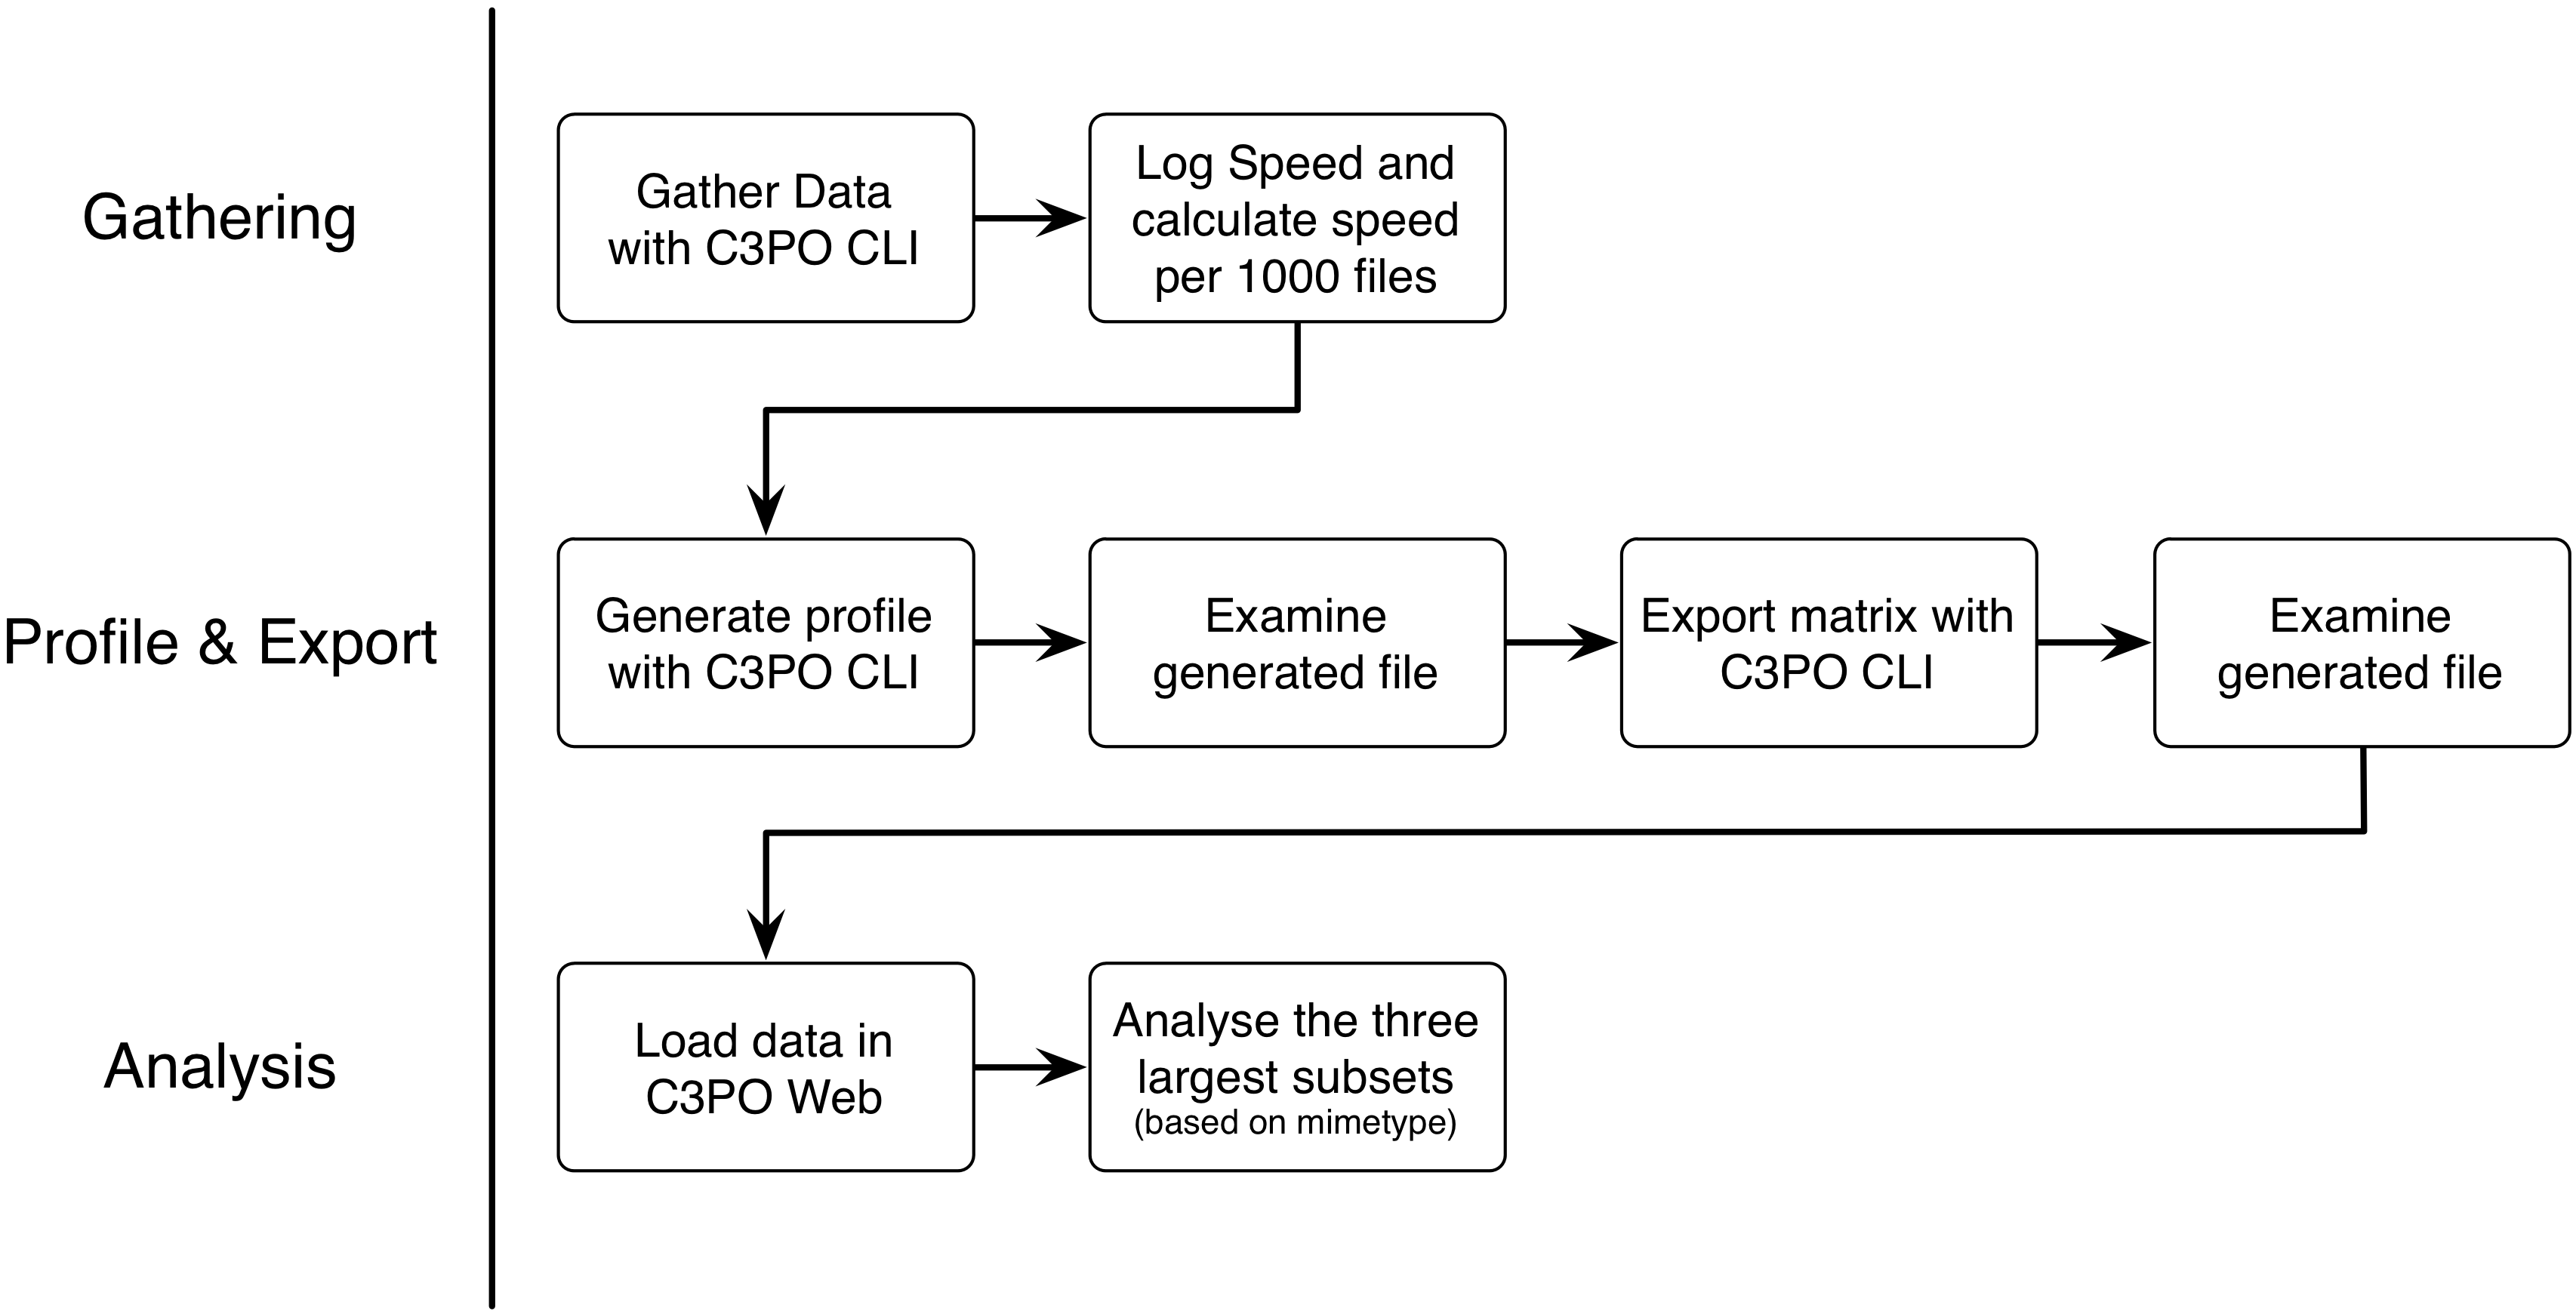
\includegraphics[width=\textwidth]{figures/usecases/experiments_flowchart.png}}
\caption{The steps for each case study}
\label{fig:exp_flowchart}
\end{center}
\end{figure}

The actual experiments conducted in each case study follow the steps of the flowchart in Figure \ref{fig:exp_flowchart}.
All of them used C3PO v0.2.0 that can be downloaded from here (\url{https://github.com/peshkira/c3po}). 

In a first step, the FITS data is gathered with the C3PO CLI application into a local instance of a MongoDB document store and the time is tracked. Afterwards the time of
the whole operation is logged as well as the time for processing 1000 files is calculated. We conduct this part of the
experiments three times with different configuration of the application in order to test the parallelisation speedup.

In a second step, we generate a XML profile with the command line application, which gets examined for errors. The size and the usefulness of the generated file is also evaluated considering the integration with other tools such as Plato and Scout. In the same step, we also generate a .CSV file containing a matrix view of all gathered data. Consequently, we examine the produced file.

In the last step we load the data within the C3PO Web application and after giving an overview of the data we analyse the three largest subsets of the collection based on the mime type.

Conducting all these steps ought to give the reader an overview of the strengths and weaknesses of the prototype implementation and what would be possible with a real world application.

\section{GovDocs1}
DigitalCorpora.org\footnote{http://digitalcorpora.org} is a website that provides digital corpora for use in computer forensics education and research.
The sites offers different file sets, network dumps, disk images and more.
For the following experiments we use the GovDocs1 file set, which contains of nearly one million freely-redistributable files that resided in the .gov domain.
The files are randomly distributed into 1000 directories with up to 1000 files in each directory and can be downloaded at \url{http://digitalcorpora.org/corp/nps/files/govdocs1/}.

\subsection{Data Description}
Forensic Innovations Inc.\footnote{http://www.forensicinnovations.com/} have provided a simple statistical report that shows some of the important characteristics of the set, which we will try to find out with C3PO and provide even more deeper insight.
The report can be found here: \url{http://digitalcorpora.org/corpora/files/govdocs1-simple-statistical-report}.
In table \ref{tab:govdoc1_general_info} general information such as file size and volume is summarised, whereas table \ref{tab:govdoc1_content} provides a summary over the content of the different files.
Note that the total sum of files in the second table is more than the number of files in the set, meaning that many files are counted twice or even more, which is not very helpful for digital preservation activities.

\begin{table}[b]
\centering
\begin{tabular}{l || c }
\hline
Characteristic & Total \\
\hline
\hline
Nr. Files & 986278 \\
File Size (KB) & 488658258 \\
Wrong File Extension & 33917 \\
Scan Time & 10:12:37 \\
\hline
\end{tabular}
\caption{General information of the GovDocs1 data set.}
\label{tab:govdoc1_general_info}
\end{table}

\begin{table}
\centering
\begin{tabular}{l || l }
\hline
Content & Total \\
\hline
\hline
  Personal/User Data & 961914\\
  Text & 727217 \\
  Document & 539100 \\
  Hypertext & 467405 \\
  Graphic Image & 464870 \\
  Macro/Script &    351781 \\
  Font & 231275 \\
  Spreadsheet & 85110\\
  Program Data  &      41616\\
  Source Code & 36580 \\
  Raw Printer Data &  26190 \\
  Database & 24820 \\
  Archived Files & 14093 \\
  Video &  3483 \\
  Email & 2007 \\
  N/A  & 882 \\
  Template & 306\\
  Program Executable & 277\\
  Presentation & 222 \\
  CAD/3D Model & 138 \\
  Game Data &15\\
  Sound/Audio & 10 \\
  Shortcut/Link & 5 \\
  Library of Functions & 2\\
  Form & 2 \\
  Encryption Key  & 1\\
\hline
\end{tabular}
\label{tab:govdoc1_content}
\caption{Content types within the GovDocs1 set as the preliminary data shows.}
\end{table}

\subsection{Experiment Preparation}
In order to conduct the experiment, all the files have to be characterised with the FITS tool.
In order to automate this task, the authors have used a workflow engine developed by the University of Manchester called Taverna\footnote{http://www.taverna.org.uk/}.
With the help of Taverna, one can create parallelised workflows that consist of number of small steps and tasks.
In this instance, the files were copied via \textit{scp} from a storage server, FITS was executed in parallel on each of the files and the output was stored on the experiments machine.

Unfortunately, the current version of FITS (v0.6) was not stable for all file types and thus it was unable to produce output for some files.
Thus all the experiments conducted on the set are done on a slightly smaller subset consisting of 945746 instead of 986278 files. The total file size of the FITS meta data was 5.37GB.

\textbf{\textit{Disclaimer}}: Due to the unpredictable behaviour of FITS on certain file types, the workflow had to be restarted numerous times.
Thus it was impossible to capture the real time for characterisation.
In the following, all time intervals that are given are only for the execution of C3PO, unless otherwise noted.
Thus any comparison with the scan time in the preliminary data should not be taken lightly.
Nonetheless, the results provided here shall give a good overview of what would be possible with a tool such as C3PO.

\subsubsection{Gathering}
In the initial test the gathering was conducted in a single thread environment. 

\begin{verbatim}
 c3po -g ~/path/to/folder/ -r -c govdocs1
\end{verbatim}

The processing of all 945746 files took more than 167 minutes.
47 files were not processed successfully due to malformed meta data files, which were caused by failures during the execution of the FITS tool.
After initial preparation and setup, processing one thousand files took 10.46 seconds on average.

The same procedure was conducted with four and 8 threads.
The speedup was 121 and 108 minutes respectively.
The average processing of one thousand files was 7.54 and 6.73  seconds respectively.
This shows more than 35\% increase in speed.
More powerful hardware (with a solid state drive disk and faster CPU) will most probably enable a speedup up to 50\% in comparison to the single threaded solution.
A next step of improvement towards the next threshold could be the parallelisation of the process on different nodes against the same document store and even distribution the store itself.
These improvements are not included as part of this work, but are possible next steps, which will enhance the process even further.

\subsubsection{Profile \& Export}
In this part of the experiment C3PO was used to generate a profile of the data processed in the previous step and to also export it.
The generated files are then inspected.

\begin{verbatim}
 c3po -p ~/path/to/output/folder -c govdocs1
\end{verbatim}

The time taken for the profile generation of the whole govdocs1 collection was 12 minutes.
The profile included 112 properties. The output file was 53 KB in size.
Considering that content profiling is not meant to be a process that delivers results instantly, these preliminary output seems to be feasible and is acceptable considering the integration with other tools over a network.

In the case that the aforementioned improvements in terms of processing are successful, then it is likely that the generation of a profile over larger content will take more time.
If the time of profile generation takes too long in such a case, a new polling strategy will have to be implemented, where an asynchronous profile generation job is submitted and the status of the result is polled by the client.

The same command was then executed with the \textit{-ie} switch, which includes the element identifiers in the profile.
The time taken was 12 minutes once again and the resulting file was 60 MB in size.
This was due to the fact that all object identifiers were included in the profile.
Since the collection is of considerable size, this shows how infeasible this option is, especially for large-scale usage.
It is helpful for demonstration purposes on smaller sized collections, but will most probably not be feasible in real world scenarios.
This part of the profile could be replaced by a special query that selects the digital objects falling into this profile.
This presents a potential problem, as the query should be agnostic to the data representation, but expressive enough to select all of the matching objects.
Furthermore, this query should be understood by any client and integrating applications, such as planning tools and digital repositories, as it will be the interface between these.
If this is can be achieved, the footprint will be once again rather small. A potential solution for this problem could be achieved by making use of the Search and Retrieve by URL - SRU\footnote{http://www.loc.gov/standards/sru/} specification that was developed by the Library of Congress.

%TODO include what was in the profile and some results.

\begin{verbatim}
 c3po -e ~/path/to/output/folder -c govdocs1
\end{verbatim}
Afterwards all the data was exported to a .csv file in a sparse matrix, with the object identifiers as rows and the properties as columns.
The generation took a little more than 2 minutes and resulted in a file of 430 MB in size.
This matrix view is very helpful to obtain an overview of the whole collection and can be used to apply some more complex filters that are not possible with the web application.
On the downside, it is questionable if this approach will scale on larger content.
While state of the art spreadsheet processors still cope with files of this size, it is highly questionable if it will be possible to open and process a much larger file.
A solution for this potential problem would be to split the exported matrix into smaller pieces and process them separately.

\subsubsection{Analysis}
In the last step the web app of C3PO was used to look at the govdocs1 content set and obtain an overview.
The following describes the set and what was possible with the tool.

C3PO revealed that the whole collection of digital objects had an overall storage size of 447.36GB of data.
This value seems to be realistic considering that FITS failed on numerous objects and the C3PO gathering process failed on some as well.
The smallest object has a size of 7 Bytes and the largest - 1.52GB.
On average all of the objects have a size of 0.48 MB with a standard deviation of 4.29 MB.
On the downside, the application did not allow the selection of the smallest and largest objects, which could be easily fixed in a next version.
In the current version, this will be only possible via the .csv export.

C3PO immediately showed that the collection consists of 46 different mime types and in addition there is one subset of conflicted mimes, which is the second most occurring.
The first 9 most occurring mime types represent nearly 80\% of the whole collection and are presented in table \ref{tab:govdocs1_mimetypes}.
The correlation between the mime type and the format of a digital object implies that both distributions are similar.
The generated distributions of C3PO validated the correlation as well.

%APPENDIX?
%The whole distribution is presented in figure

\begin{table}[h]
\centering
\begin{tabular}{l || l }
\hline
Mime Type & Count \\
\hline
\hline
 application/pdf & 224495 \\
 conflicted 	& 160354 \\
 text/html		&  138161 \\
 image/jpeg	&  106714 \\
 text/plain		& 93280 \\
 application/mswod & 73282 \\
 application/vnd.ms-excel & 42877 \\
 image/gif		& 35292 \\
 text/xml		& 25347\\
 \hline
\end{tabular}
\caption{The 9 most occurring mime types within the GovDocs1 set as C3PO showed.}
\label{tab:govdocs1_mimetypes}
\end{table}

The next interesting observation was the creation date distribution of the content set.
The following table \ref{tab:govdocs1_created} presents it.
The total of the files in this distribution is much less than the total of the collection, because of the data sparsity.
Nonetheless, there are some interesting observations that can be made out of this distribution.
Firstly, the objects created between 2003 and 2008 are much more than the rest.
This can be related to the fact that data production does not increase constantly, but rather exponentially during the years.
Although this conclusion might be biased as the data may not be sufficient to back it up.
Secondly, it is very interesting that the data created in 2009 is  less than some data created during the 90s.
Thirdly, there is one small subset that is gathered in year '-1'.
This is clearly a faulty measure provided by some of the characterisation tools bundled in FITS, which proves the point of the importance of meta data quality.
Last but not least, one subset was created in 1910, which is rather peculiar and is most probably related to bad data quality.

\begin{table}[h]
\centering
\begin{tabular}{l || l }
\hline
Created Date & Count \\
\hline
\hline
2004 	& 38246 \\
2007 	&  37526 \\
2008		&  37152 \\
2006 	&  36276 \\
2005		&  35780 \\
2003		&  35204 \\
2002		&  26327 \\
2001		&  20134 \\
2000		& 15976 \\
1999		& 13006 \\
1998		&  9334 \\
1997		&  5597 \\
2009		&  5357\\
1996		&  2725\\
-1		&  2703\\
1910		&  2052\\
Rest		&  6362\\
 \hline
\end{tabular}
\caption{The 9 most occurring mime types within the GovDocs1 set as C3PO showed.}
\label{tab:govdocs1_created}
\end{table}

\paragraph{Portable Document Format}
Adding a new mime type based filter showed that the 224495 application/pdf files in the govdocs1 set consisted of three different PDF formats (PDF, PDF/A and PDF/X) with more than 10 different versions.
This is about 28\% of the storage size  needed for the whole collection.

In a next step, the validity and well-formedness of the documents was examined.
90\% of these documents were valid, nearly 10\% were invalid and less than 1\% were unknown.
Almost all documents were well-formed. About 1\% were not and once again less than 1\% were unknown.
Considering only files with unknown validity, made it possible to conclude that  the unknown files in terms of validity and wellformedness were exactly overlapping.
Because of this fact, they are excluded of the following observations.

C3PO showed that all valid pdf documents were also well formed.
However, 8\% of all well-formed pdf objects were invalid.
None of these 8\% were in format PDF/X, which implies that all PDF/X formatted objects were reported to be both valid and well-formed.

Selecting the subset of invalid and not well-formed documents, which were about 1\% of the whole pdf collection, showed that it consists only of PDF documents (in all versions from 1.0 to 1.6).
C3PO also provided a list of so called 'evil' applications that created these malformed files.
Most were created by different versions of Acrobat Distiller.

Finally the distribution of the properties 'is rights managed' and 'is protected' were generated.
It turns out that only 81 pdf documents had rights data associated with them, whereas 97\% didn't have any.
For about 2\% it was unknown.
The protected pdfs were many more in comparison - about 4\%.
Again 2\% were unknown and the rest were not protected.
Eight objects were conflicted in terms of protection.
All of these were invalid and not well-formed. Two had the format PDF 1.4 and six PDF 1.6.

The analysis of this type of objects was quite easy and the tool enabled the user to drill down and find out interesting facts about this subset.

\paragraph{Conflicted}
Examining the objects with conflicted mime type values with C3PO proved to be rather hard and showed room for optimisation and enhancement in the future versions of C3PO.
Besides of the storage size statistics the information was not very helpful.
The storage size of all 160353 objects was about 81GB.
All the formats in the subset were also conflicted and only versions were shown, which was not enough information to gain an overview of the conflicted subset (the second highest in the whole set).
An idea was to take a look at the creating applications and to obtain a rough overview of the type of documents in this subset.
However, 99\% of these were unknown.

In terms of validity and wellformedness, the following observations were made.
For 48\% of the subset both these properties were unknown.
All 20\% of the valid objects in this subset were also well formed.
The other 32\% of invalid objects contained both well formed and not well formed objects in ratio 3 to 2.

All this showed, that it will be helpful to a planner to see a list of conflicted values or some kind of weighted distribution. 
Additional filters over these would also be helpful.
Furthermore, it will be beneficial to apply special rules that resolve the conflicts in cases where the characterisation tools provide conflicts for similar formats (e.g. text/xhtml, text/xml).

\paragraph{JPEG}
As there is a second case study, conducted over data from a web archive which will naturally include many html files, we skip the third most common mime type (text/html) in this collection and focus on the next one -  image/jpeg.

This subset consists of 106714 objects or about 11\% of the whole set.
The storage space needed for this subset is about 34GB.

Two formats were identified within this subset (JPEG and EXIF) with more than 10 different versions.
80\% of the files were valid and wellformed. Only 3 objects were invalid.
The rest was unknown both in terms of validity and wellformedness.

The JPEG files presented 95\% of the subset and most of them had YCbCr colorspace.
The rest were unknown.

The EXIF files were significantly smaller (a bit more than 4\%).
For most of them the colorspace was unknown.
The rest were RGB-colored images.

Other interesting data provided by FITS were the GPS coordinates of some images.
Unfortunately, C3PO is not able to make use of these in order to visualise them.
Nonetheless, an overview of the objects having such meta data could be an interesting asset in a digital preservation activity considering a scenario where such meta data has to be kept after a preservation action is conducted. 

\section{Web Archive Data}
The Danish State University Library\footnote{http://en.statsbiblioteket.dk} (SB) has a mandate to maintain the whole danish web archive.
This includes every website of the Danish domain (.dk top-level domain), all web content hosted by danish companies, all content produced by Danish and more.
Currently the archive has content with more than seven billion objects with size in the order of petabytes. The growth of the archive is expected to rise exponentially during the next decade.

\subsection{Data Description}
In collaboration with the University of Technology in Vienna, the SB has shared the FITS metadata of a subset of the web archive harvested over the last eight years.
The files were selected randomly and contain not only HTML documents but all related content, such as stylesheets, script files, image material, etc.
Due to the volume of the data, even the administrators of the archive do not have an overview of the data they possess.
In the following we analyse 958,953 FITS files with an overall size of 4.18GB.

\subsection{Experiment Preparation}
In this case, the FITS files were generated by the SB. They used an extended version of FITS, which was provided by the University of Technology in Vienna.
This version deactivated the JHOVE tool for html files, due to its known bad performance and  included another tool that provides some more information about html content.
Once again, all time measurements provided in the following solely include the time that C3PO needed for execution, unless otherwise stated.

\subsection{Experiment}
Here we undergo the same steps as with the previous experiment and measure the times needed for gathering, processing and profiling.
Afterwards, an overview analysis over the content is done, in order to test the functionality and limitations of the prototype implementation and the proposed profiling approach.

\subsubsection{Gathering}
The processing was done with 8 threads and took 178 minutes for  all 958,953 files. 316 files were not processed successfully, due to a bug in C3PO. The average processing time of 1000 files took 10.92 seconds. 

\subsubsection{Profile \& Export}
Generating the machine readable profile took 13.5 minutes. The resulting file was 700K in size. Repeating the profiling procedure with included object identifiers, took nearly the same time and resulted in a file of almost 200 MB size. This rather large increase in file size shows how infeasible this strategy would be at even larger scales.

A problem that was revealed by the profile was that the datatype of some of the characteristics were not correctly identified. This resulted in bogus aggregations for some of the numeric properties. Further investigation will be needed in order to determine whether this was caused by bad meta data or bad implementation in C3PO.

The export of the sparse matrix took about 2 minutes and 40 seconds and resulted in a 580MB file.

\subsubsection{Analysis}
Since there is no overview or ground truth data about the archive, we suspect to see that the web archive consists of mostly html documents, text documents (the stylesheets and scripts) as well as images. It is highly possible that there are a lot of conflicts, as the tools bundled in FITS often do not agree whether a file is xml, html or a mixture of both.
Another assumption is that the average file size is around 0.2MB, which means that the overall size of the analysed web archive data should be a little less than 200GB.

Looking at the data with C3PO, revealed the following:

In terms of size, the assumptions were wrong by a factor of almost 8. The analysed web archive data has an overall size of  26GB. The average file size is 0.03MB with a standard deviation of 0.66MB. The smallest file within the data was 1B and the largest 201.73MB. This proves how difficult it is to predict even the size of such a heterogeneous collection, not to mention other more complex characteristics.

The following table gives a distribution of the mime types identified within the collection.

\begin{table}[h]
\centering
\begin{tabular}{l || l }
\hline
Mime Type & Count \\
\hline
\hline
 image/jpeg & 306654 \\
 text/html 	& 250316 \\
 image/gif		&  199147 \\
 conflicted	&  104722 \\
 text/plain		& 52379 \\
 image/png & 23878 \\
 application/pdf & 7055 \\
 text/xml		& 6620\\
 application/octet-stream & 2096 \\
 image/x-ico	& 1324\\
 rest			& 4447\\
 \hline
\end{tabular}
\caption{The most represented mime types identified within the web archive collection as C3PO showed.}
\label{tab:webarchive_mimetypes}
\end{table}

\paragraph{Hypertext Markup Language}
Observing this mime type distribution shows that the initial assumptions are mostly correct. At a first glance, It is curious that there are more images than html files. The reason for that could be the fact that the fourth most occurring mime type category is \textit{conflicted}. Since such a high number of conflicts was expected due to known problems with FITS, we examine the conflicted subset first. As the formats were also \textit{conflicted}, the only clue that C3PO was able to provide were the format versions. 50\% had version '1.0'. Since many formats could have this version, the PUIDs of the subset were examined. It revealed that all of this 'conflicted' files had one of the following: \textit{fmt/101}, \textit{fmt/102}, \textit{fmt/96}. A quick check with the PRONOM registry showed that these are XML and HTML formats. From this two conclusions can be drawn. Firstly, it was fairly easy to identify the 'conflicted' documents by crossmatching the format version with other properties, such as the PUID. Secondly, the problems with the FITS conflict resolution for XML and HTML were shown. Another 30\% of the same document subset had version \textit{4.01} which is a HTML version. Looking at the raw meta data confirmed this assumption. If we sum up the correctly identified HTML documents and the ones that are \textit{conflicted} but were proven to be html, then the initial assumption of having mostly HTML files will be correct.

C3PO provides a simple pre- and post processing mechanism that is used during the gathering phase, which might offer a solution to such problems caused by conflicted data. Writing a simple post processing rule that checks the conflicted values of the format property and overwriting them, if and only if they are XML and HTML before storing the meta data in this particular example. There are two problems with this solution. First, the current implementation does not allow dynamic processing rule binding, which implies that the rules have to be precompiled and poses an inconvenience to the user. Second, making use of such a rule is a rather dangerous decision and requires the knowledge of an expert who understands the data well and the implications in case of creating a wrong rule.

Concentrating on the correctly identified html subset (the second group in the mime type table) showed the following.
The size of this subset was a bit more than 3GB. 94\% of the documents were not valid opposed to less than 1\% valid. The rest were unknown. Wellformedness revealed that 57\% were not well structured html documents, whereas 38\% were well formed.

\paragraph{JPEG}
The 306654 JPEG objects amounted to 32\% of the whole set. Their overall size was almost 8GB.
Most of the images were formatted with version '1.01' (48\%), closely followed by format version '1.02' (41\%). The rest of the format versions were distributed around 10 other versions.

82\% were valid and wellformed. Almost 18\% were unknown in terms of validity and well-formedness and the very small rest were either not valid, not well-formed or both.

Also 82\% were had the YCbCr colorspace and nearly 18\% had RGB. At first the authors thought that these are the same subsets as the ones in the validity and wellformedness experiments. However, a short analysis showed that this conclusion cannot be drawn.

Once again, the creating date was not extracted out of many files. Most of the files (for which it was extracted) were created between 2003 and 2007.

\paragraph{Graphics Interchange Format}
The size of this subset was 1GB with an average file size of 0.01MB, which is usual for such web content.
97\% of the GIF (animated) images were formatted with the newer enhanced version - 89a, whereas the rest had the older 87a version. Almost all of them were valid and well-formed and a very small subset of objects (566) were both invalid and not well-formed.

As expected most of them were compressed with LZW\footnote{http://en.wikipedia.org/wiki/Lempel-Ziv-Welch}, which is a lossless data compression scheme and is common for GIF images. Nonetheless, there were 4 GIFs that had conflict in compression, which is rather strange. It would be interesting to look at the originals and check, why the conflict is reported. Unfortunately, the original content cannot be obtained in this case.

Again, only a few had associated creation meta data.

\section{Observations}
In this section we observe the outcomes of the experiments and try to give an objective evaluation of the C3PO prototype tool.

Altogether, the experiments showed, that C3PO can be rather useful in giving a complete overview of the identification data of rather large collections. In cases, such as the web archive data, where it is rather hard to get an idea what content there is, the identification data, such as mime types, formats and format versions, gives a rather valuable insight into the data. Even in cases where there were conflicts, it was still possible to figure out the type of content by creating some filter conditions. Considering that web archives, currently try to preserve web content by ensuring the bit streams are kept in tact and that access is still possible, the information that C3PO provides is rather useful. 

The other use case showed that in cases of documents or images, where different preservation actions might be chosen, not only a good overview of the identification data is given, but also some specific information about some characteristics can be aggregated and displayed.

Nonetheless, there were two big issues regarding the meta data and thus the quality of C3PO. For one the data sparsity is a huge problem, as it often makes it hard to distinguish between format homogeneous subsets. What is more, the quality of the data is very important. Even if a measurement is reported, there is almost no way of knowing if this is the correct measurement, or a bug in the characterisation process.

Scalability was shown to be feasible for collections of size up to a million objects on a single commodity machine. Using  better hardware will probably allow some vertical scalability but only to a certain point. The next logical step is taking advantage of the horizontal scalability capabilities of the back end, which still have to be tested. What is more, the gathering process can be also distributed on more nodes, in order to improve performance.

As far as the machine readable profile is concerned, it was shown that its creation is feasible. However, its structure and usefulness has to be evaluated by integration with other software components. Two potential problems were shown by these experiments. First, including a long list of identifiers is a solution which will not scale due to the resulting file size.
Second, it is questionable, whether or not the inclusion of all known properties in aggregated form is needed.

Export of the data in a sparse matrix was shown to be rather fast and helpful for the user. However, this approach will most probably not scale for all data on larger collections, as spreadsheet tools will most likely have problems handling such big files. Nonetheless, exporting only subsets of the data can be rather helpful to a preservation
expert. Another question to look at in future work is the use case scenarios of the matrix and consider adding new features to c3po that can cover these use cases.

The current implementation allows to filter or correct some of the meta data that might be wrong during the processing phase. By implementing some pre-processing rules, it will be possible to enhance the quality of the data (e.g. XML/HTML identification). However, this task might lead to faulty results, as such assumptions should not be done lightly. Also the dynamic binding of such rules is not yet supported.

When looking at the selected samples, one potential pitfall was found. None of the proposed algorithms is able to deterministically select outliers in homogeneous sets, which is a hint for a further optimisation.

The current prototype implementation provides visualisations for each characteristic in form of histograms. Nonetheless, it was shown that it will be helpful to combine some of the characteristics in other types of visualisations (e.g. scatterplots or bubble charts). In the case of GPS data or image resolution data, this could make a lot of sense.

Filtering showed that in a few easy steps it is possible to find some interesting facts about the data. Enhancing the filtering mechanism further, will be even more helpful to a planner. For example inverting the condition or adding a logical 'OR' to the conditions might be helpful.